\documentclass[]{article}

\usepackage{graphicx}
\usepackage{float}

%opening
\title{Client-Side Many-Valued \protect\\ Context Scaling \protect\\ Documentation}

\begin{document}

\maketitle

\newpage
\section{Upload}
\begin{figure}[H]
	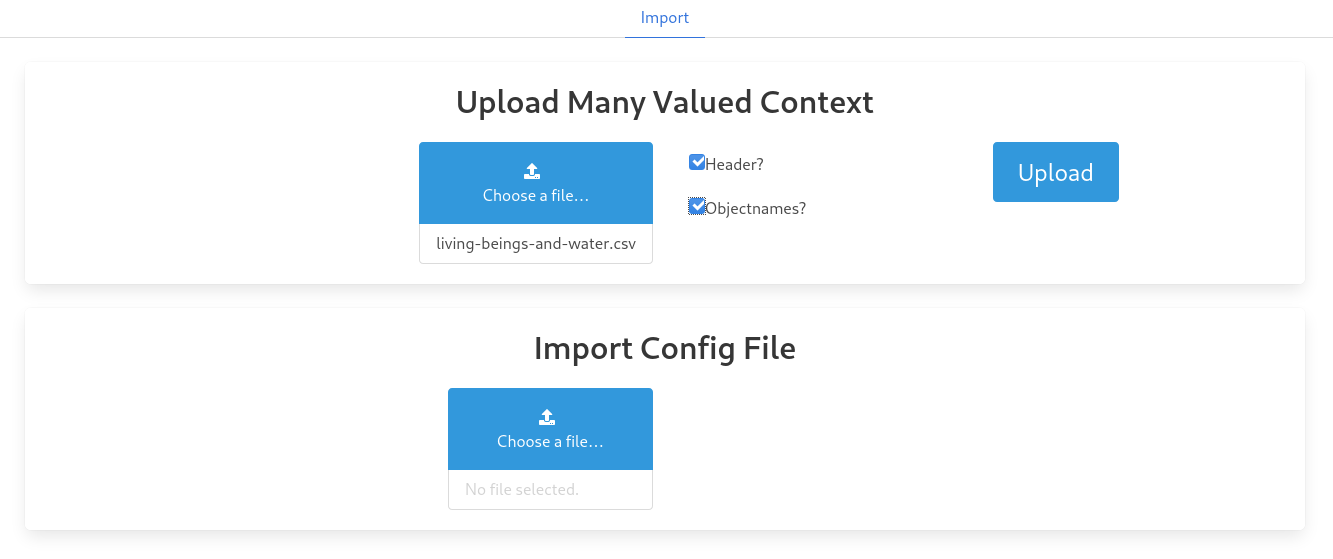
\includegraphics[width=\linewidth]{images/upload.png}
	\caption{The panel to select files}
	\label{fig:p2}
\end{figure}
\subsection{Features}
\begin{itemize}
    \item The topmost bar allows for navigation and is updated with new panels whenever they get accessible.
	\item Select any local .csv file with a mv-context.
    \item There is the option to include a "header" (first line in file) with attribute names.
    \item "Objectnames" can be included in the first column of the file.
    \item To upload the file, click the "Upload"-button.
    \item Additionally, you can edit already scaled contexts by importing config files (generated by the last panel in this document)
\end{itemize}

\section{Attribute-Selection}
\begin{figure}[H]
	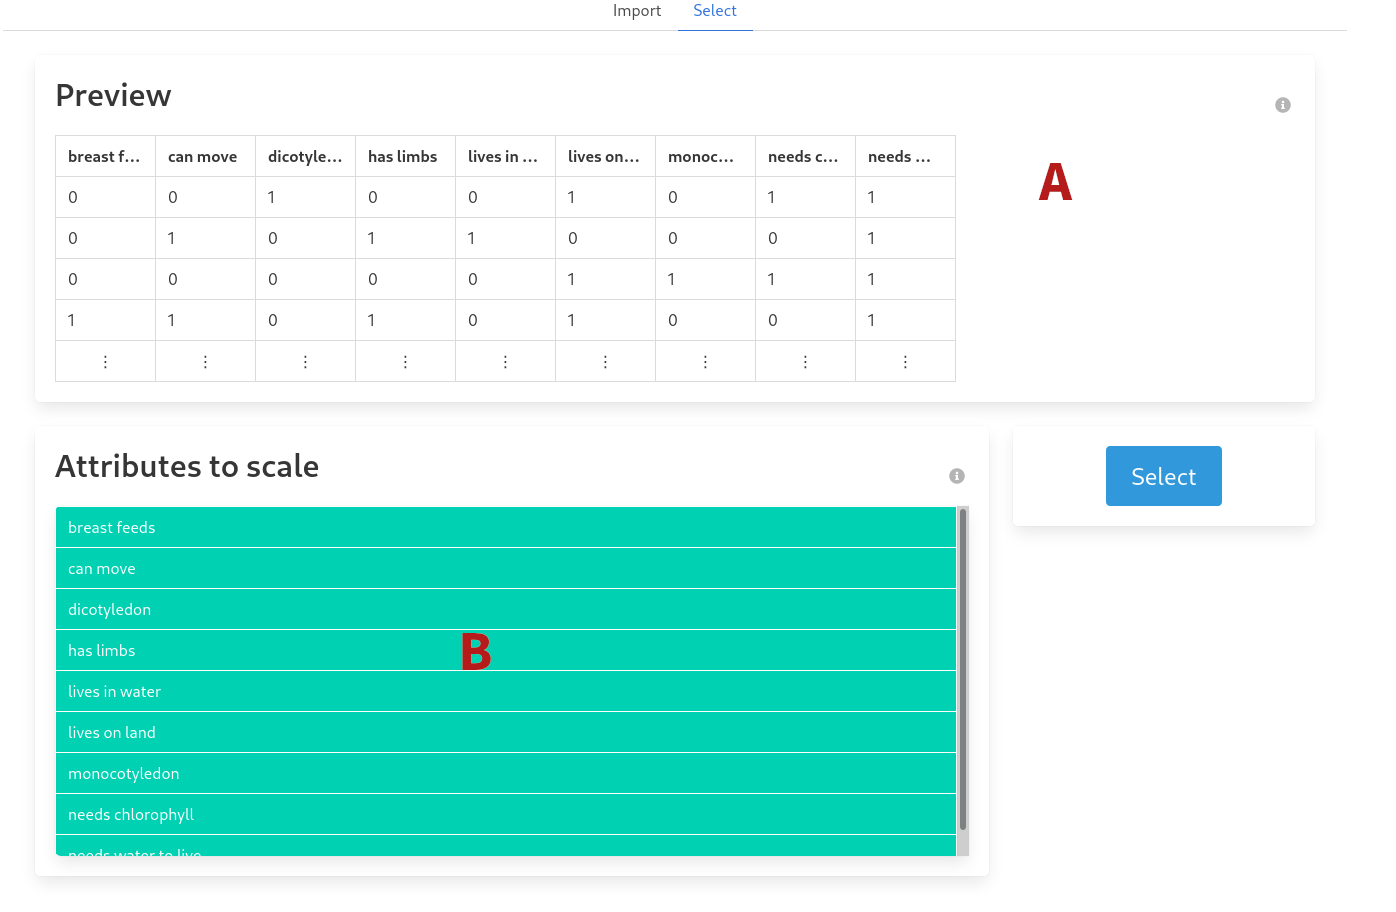
\includegraphics[width=\linewidth]{images/selection.png}
	\caption{The panel to select attributes}
	\label{fig:p1}
\end{figure}
\subsection{Features}
\begin{itemize}
    \item The top half displays a preview of the uploaded data.
    \item The bottom half allows for attributes to be selected for scaling. By default all attributes are selected (green) but can be unselected (white) with a click.
    \item By holding down the mouse button  multiple attributes can be de-/selected.
    \item Click "Select" to manually scale the chosen attributes.
\end{itemize}

\section{Scaling}
\begin{figure}[H]
	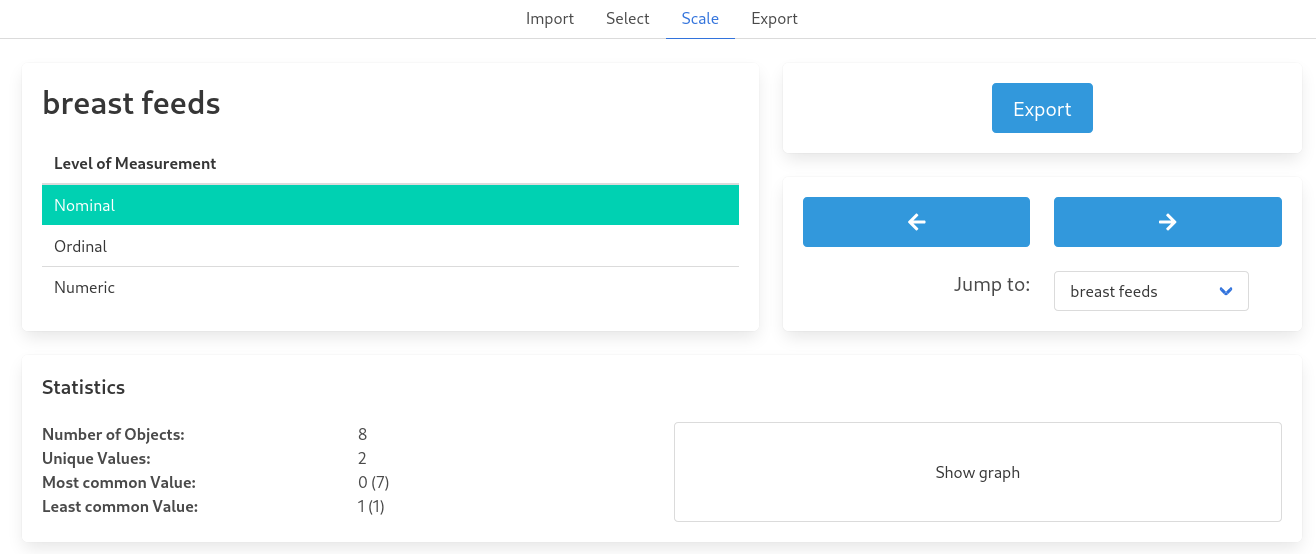
\includegraphics[width=\linewidth]{images/nominal.png}
	\caption{The panel to scale attributes}
	\label{fig:p3}
\end{figure}
\subsection{Features}
\begin{itemize}
    \item The top left half allows for the selection of the scaling method for the current attribute (title). Based on the corresponding data some options may not be selectable.
    \begin{itemize}
        \item Subsequent sections will go into "Numeric" and "Ordinal" scaling. "Nominal" scaling is done automatically.
    \end{itemize}
    \item The top right half allows for the "Export" of the scaled context. All unchanged attributes may be scaled nominally.
    \item Below the "Export" one can change the current attribute.
    \item Each scaling method shows "Statistics" relevant for the scaling and the option for a graph.
\end{itemize}

\section{Scaling Graph}
\begin{figure}[H]
	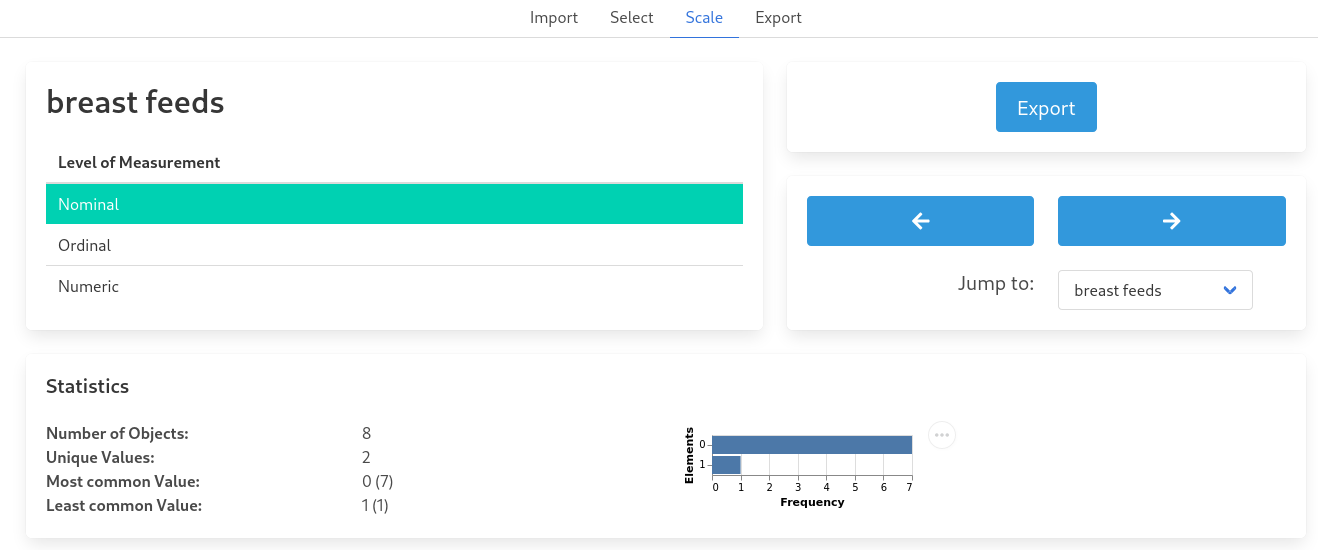
\includegraphics[width=\linewidth]{images/nominal_graph.png}
	\caption{The panel to select attributes}
	\label{fig:p4}
\end{figure}
\subsection{Features}
\begin{itemize}
    \item By clicking the button a temporary graph is generated. The graph will disappear upon changing the scaling method or upon changing the current attribute and has to be generated again.
\end{itemize}

\newpage
\section{Ordinal Scaling}
\begin{figure}[H]
	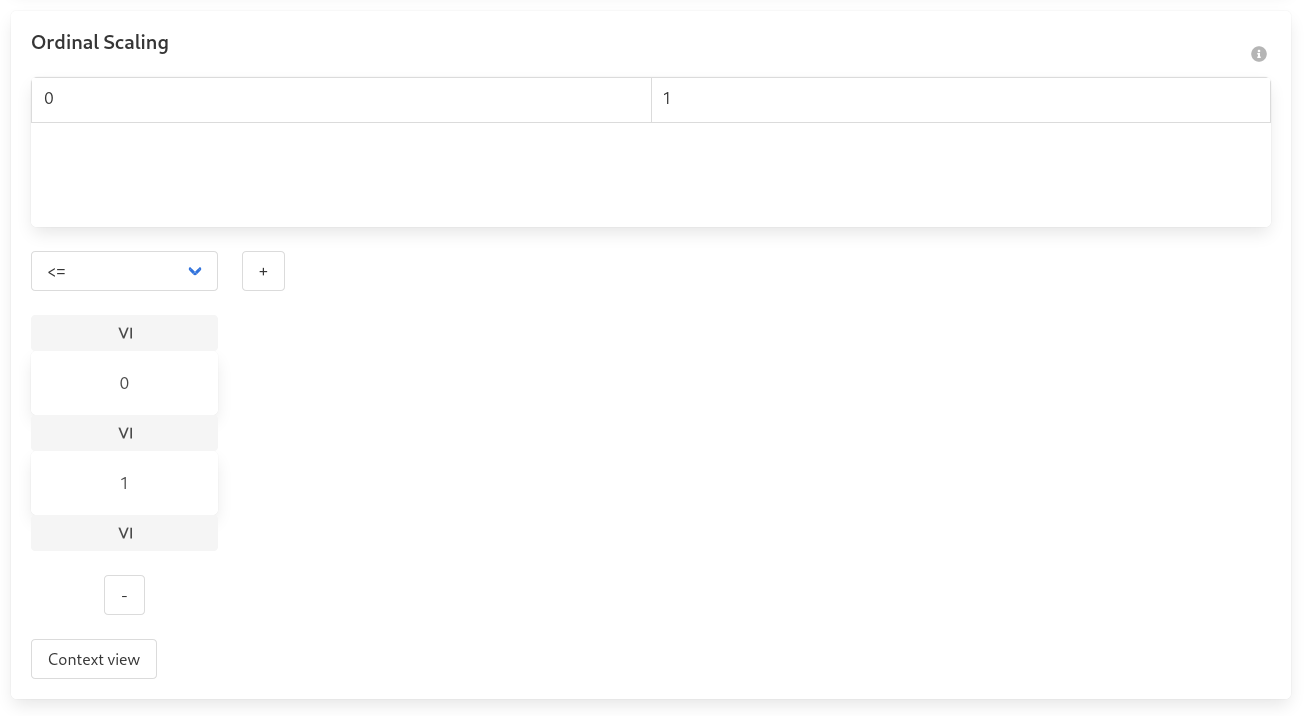
\includegraphics[width=\linewidth]{images/ordinal.png}
	\caption{The panel to scale ordinal attributes}
	\label{fig:p5}
\end{figure}
\subsection{Features}
\begin{itemize}
    \item The default option to perform ordinal scaling is to build orders from the possible values.
    \item The box on top of the panel contains each different value the attribute has.
    \item Below a new order can be created either by clicking the "+" or by dragging values from the box above on the "+"-button.
    \begin{itemize}
        \item Each order has a drop-down menu were an order relation can be selected.
        \item By dragging values onto the grey areas the value is inserted into the order.
        \item Values can also be dragged out of the order or into different positions by dragging the white box of the corresponding value.
    \end{itemize}
    \item The "Context view"-button transforms the current orders into a context and changes the panel.
\end{itemize}

\section{Ordinal Context Scaling}
\begin{figure}[H]
	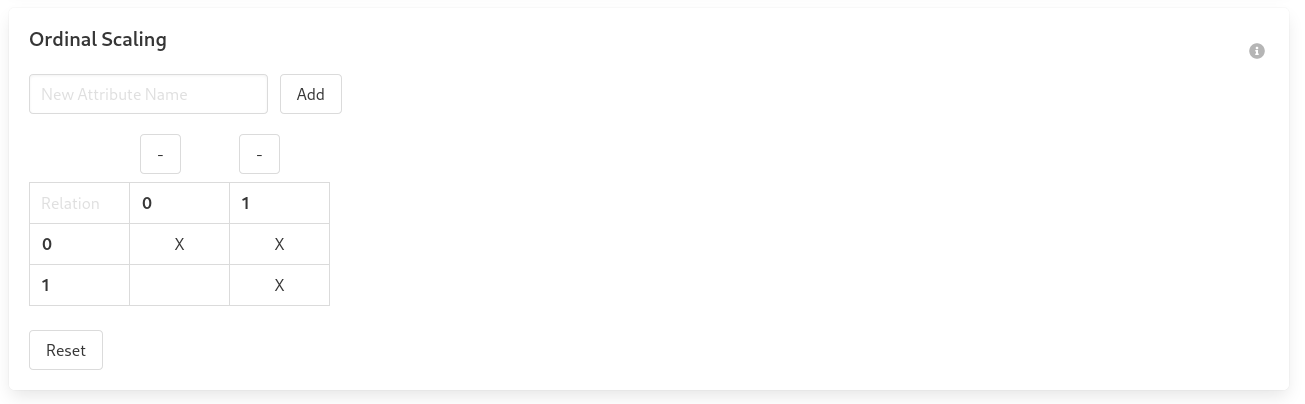
\includegraphics[width=\linewidth]{images/ordinal_ctx.png}
	\caption{The second panel to scale ordinal attribute}
	\label{fig:p6}
\end{figure}
\subsection{Features}
\begin{itemize}
    \item Per default the generated context is quadratic and contains all orders previously built.
    \item New attributes can be generated by writing their name in the topmost input field and clicking "Add". Clicking the "-" removes the attribute below it.
    \item Attributes and objects can be sorted with drag and drop.
    \item The top left corner allows to name the relation used which is purely cosmetic.
    \item To swap a relation between " " and "x" click the corresponding field.
    \item "Reset" discards all changes done to the context and return to the previous panel with all orders built before.
\end{itemize}

\section{Numeric Scaling}
\begin{figure}[H]
	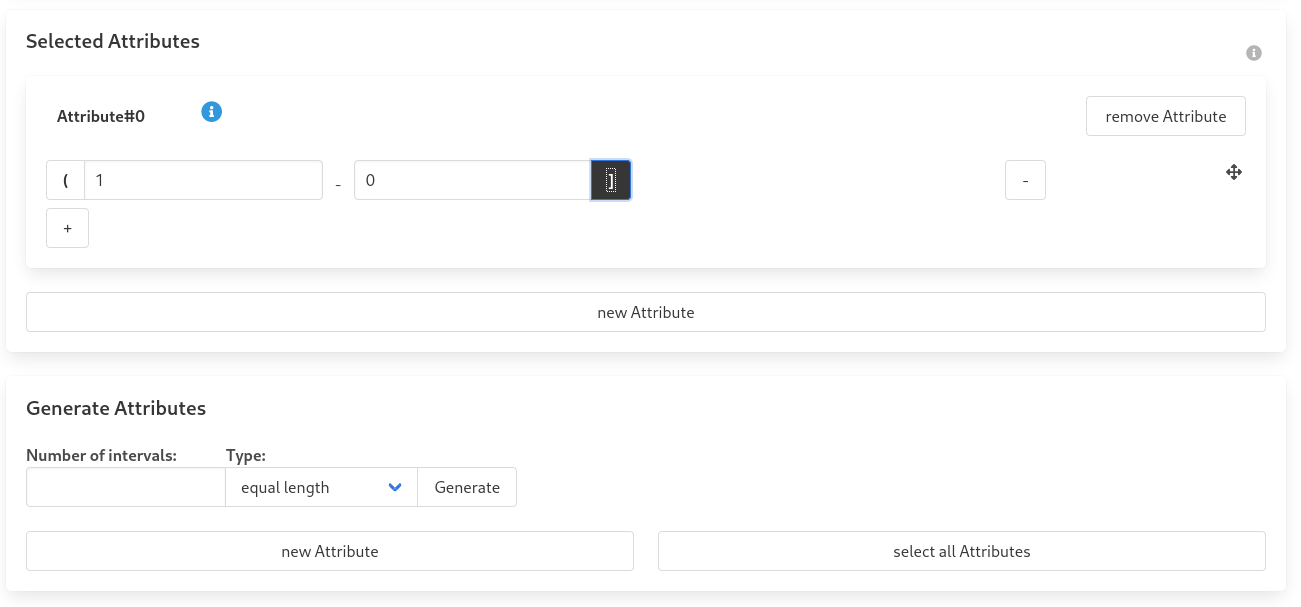
\includegraphics[width=\linewidth]{images/numeric.png}
	\caption{The panel to scale numeric attributes.}
	\label{fig:p7}
\end{figure}
\subsection{Features}
\begin{itemize}
    \item The upper panel contains all selected attributes.
    \begin{itemize}
        \item "new Attribute" and "remove Attribute" add/delete attributes. 
        \item The attribute name can be clicked and written in to change it.
        \item "+" and "-" add/delete intervals from an attribute.
        \item A value is added to an attribute if it is contained in one of its intervals. The interval can be toggled to be open ("(") and closed ("]") by clicking the brackets.
        \item Intervals can moved to other attributes by drag and drop.
    \end{itemize}
    \item The lower panel generates attributes.
    \begin{itemize}
        \item By clicking "Generate" the written number of intervals is generated by the selected method from the drop-down menu.
        \item Those attributes must be selected to be used by clicking "Select" or "Select all". Selected Attributes are moved to the upper half.
    \end{itemize}
\end{itemize}

\section{Export panel}
\begin{figure}[H]
	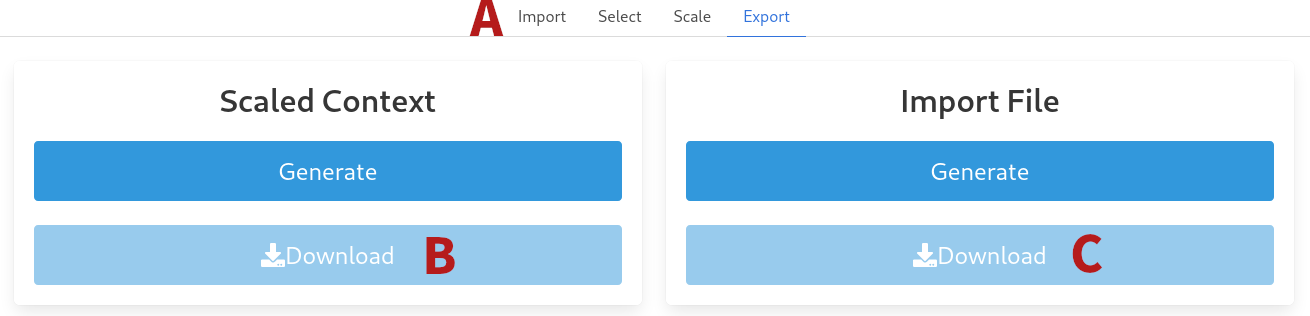
\includegraphics[width=\linewidth]{images/export.png}
	\caption{The panel to export the scaled context}
	\label{fig:p4}
\end{figure}
\subsection{Features}
\begin{itemize}
    \item By clicking the corresponding button an import file and a scaled context can be "generated".
    \item The scaled context applies all chosen scales to the selected attributes and outputs the context in "Burmeister"-format.
    \item The import file consists of a .json file with the current state of the application. This file can later be used to change the different scaling methods applied to the attributes or to change the selected attributes.
\end{itemize}

\end{document}
